%%%%%%%%%%%%%%%%%%%%%%%%%%%%%%%%%%%%%%%%%%%%%%%%%%%%%%%%%%%%%%%%%%%%%
% PREAMBLE
%%%%%%%%%%%%%%%%%%%%%%%%%%%%%%%%%%%%%%%%%%%%%%%%%%%%%%%%%%%%%%%%%%%%%
%
% The following two commands will generate a PDF that follows all the requirements for submission
% and peer review.  Uncomment these commands to generate this output (and comment out the two lines below.)
%
% DOUBLE SPACE VERSION FOR SUBMISSION TO THE AMS
%\documentclass[12pt]{article}
%\usepackage{ametsoc}
%\linenumbers
%
% The following two commands will generate a single space, double column paper that closely
% matches an AMS journal page.  Uncomment these commands to generate this output (and comment
% out the two lines above. FOR AUTHOR USE ONLY. PAPERS SUBMITTED IN THIS FORMAT WILL BE RETURNED
% TO THE AUTHOR for submission with the correct formatting.
%
% TWO COLUMN JOURNAL PAGE LAYOUT FOR AUTHOR USE ONLY
\documentclass[10pt]{article}
\usepackage{ametsoc2col}
%\usepackage{dblfloatfix}

%
%%%%%%%%%%%%%%%%%%%%%%%%%%%%%%%%%%%%%%%%%%%%%%%%%%%%%%%%%%%%%%%%%%%%%
% ABSTRACT
%
% Enter your Abstract here
%%%%%%%%%%%%%%%%%%%%%%%%%%%%%%%%%%%%%%%%%%%%%%%%%%%%%%%%%%%%%%%%%%%%%
\newcommand{\myabstract}{There's lots of noisy GPS data. Here's how you should smooth it.}
%
\begin{document}
%
%%%%%%%%%%%%%%%%%%%%%%%%%%%%%%%%%%%%%%%%%%%%%%%%%%%%%%%%%%%%%%%%%%%%%
% TITLE
%
% Enter your TITLE here
%%%%%%%%%%%%%%%%%%%%%%%%%%%%%%%%%%%%%%%%%%%%%%%%%%%%%%%%%%%%%%%%%%%%%
\title{\textbf{\large{Smoothing Noisy GPS Data}}}
%
% Author names, with corresponding author information. 
% [Update and move the \thanks{...} block as appropriate.]
%
\author{\textsc{J. J. Early,}
				\thanks{\textit{Corresponding author address:} 
				Jeffrey J. Early, NorthWest Research Associates, 
				4118 148th Ave NE, Redmond, WA 98052. 
				\newline{E-mail: jearly@nwra.com}}\quad\textsc{A. Sykulski}\\
}
%
% Formatting done here...Authors should skip over this.  See above for abstract.
\ifthenelse{\boolean{dc}}
{
\twocolumn[
\begin{@twocolumnfalse}
\amstitle

% Start Abstract (Enter your Abstract above.  Do not enter any text here)
\begin{center}
\begin{minipage}{13.0cm}
\begin{abstract}
	\myabstract
	\newline
	\begin{center}
		\rule{38mm}{0.2mm}
	\end{center}
\end{abstract}
\end{minipage}
\end{center}
\end{@twocolumnfalse}
]
}
{
\amstitle
\begin{abstract}
\myabstract
\end{abstract}
\newpage
}
%%%%%%%%%%%%%%%%%%%%%%%%%%%%%%%%%%%%%%%%%%%%%%%%%%%%%%%%%%%%%%%%%%%%%
% MAIN BODY OF PAPER
%%%%%%%%%%%%%%%%%%%%%%%%%%%%%%%%%%%%%%%%%%%%%%%%%%%%%%%%%%%%%%%%%%%%%
\section{Introduction}



%%%%%%%%%%%%%%%%%%%%%%
%
\section{B-Splines}
%
%%%%%%%%%%%%%%%%%%%%%%

A B-spline, or basis spline, of order $K$ is a piecewise polynomial function defined with respect to knot points. The terminology here is confusing, but generally seems to be that a B-spline of \emph{order} $K$, is a piecewise polynomial of \emph{degree} $S=K-1$. That means that a $4$th order B-spline is a piecewise cubic polynomial. The \emph{knot points} define the location where the polynomials meet. Continuity is maintained to as high of order as possible. So a $K=1$ B-spline is a piecewise constant function with value $1$ between two knot points, while $K=2$ B-spline forms a continuous triangle function with a piecewise constant first derivative (see figure \ref{bsplines}).

\begin{figure}[t]
  \noindent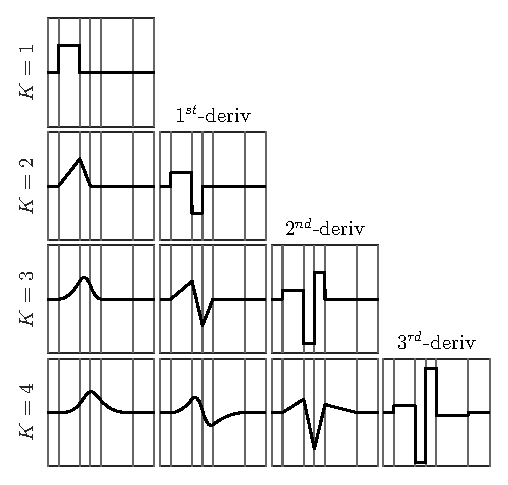
\includegraphics[width=39pc,angle=0]{bsplines}\\
  \caption{This shows an example B-spline and its derivatives (columns) for orders $K=1..4$ (rows).}
  \label{bsplines}
\end{figure}

%%%%%%%%%%%%%%%%%%%%%%
%
\section{Smoothing Spline}
%
%%%%%%%%%%%%%%%%%%%%%%


%\begin{acknowledgment} 
%Start acknowledgments here.
%\end{acknowledgment}
%
%% Use appendix}[A], {appendix}[B], etc. etc. in place of appendix if you have multiple appendixes.
%\ifthenelse{\boolean{dc}}
%{}
%{\clearpage}
%\begin{appendix}
%\section*{\begin{center}Appendix Title Is Entered Here (Primary heading)\end{center}}
%\subsection{First appendix secondary heading}
%
%\subsection{Second appendix secondary heading}
%
%\subsubsection{First appendix tertiary heading}
%
%\subsubsection{Second appendix tertiary heading}
%
%\paragraph{First appendix quaternary heading}
%
%\paragraph{Second appendix quaternary heading}
%
%\end{appendix}
%
%% Create a bibliography directory and place your .bib file there.
%% -REMOVE ALL DIRECTORY PATHS TO REFERENCE FILES BEFORE SUBMITTING TO THE AMS FOR PEER REVIEW
%\ifthenelse{\boolean{dc}}
%{}
%{\clearpage}
%\bibliographystyle{ametsoc}
%\bibliography{references}
%
%%%%%%%%%%%%%%%%%%%%%%%%%%%%%%%%%%%%%%%%%%%%%%%%%%%%%%%%%%%%%%%%%%%%%%
%% FIGURES-REMOVE ALL DIRECTORY PATHS TO FIGURE FILES BEFORE SUBMITTING TO THE AMS FOR PEER REVIEW
%%%%%%%%%%%%%%%%%%%%%%%%%%%%%%%%%%%%%%%%%%%%%%%%%%%%%%%%%%%%%%%%%%%%%%
%\begin{figure}[t]
%  \noindent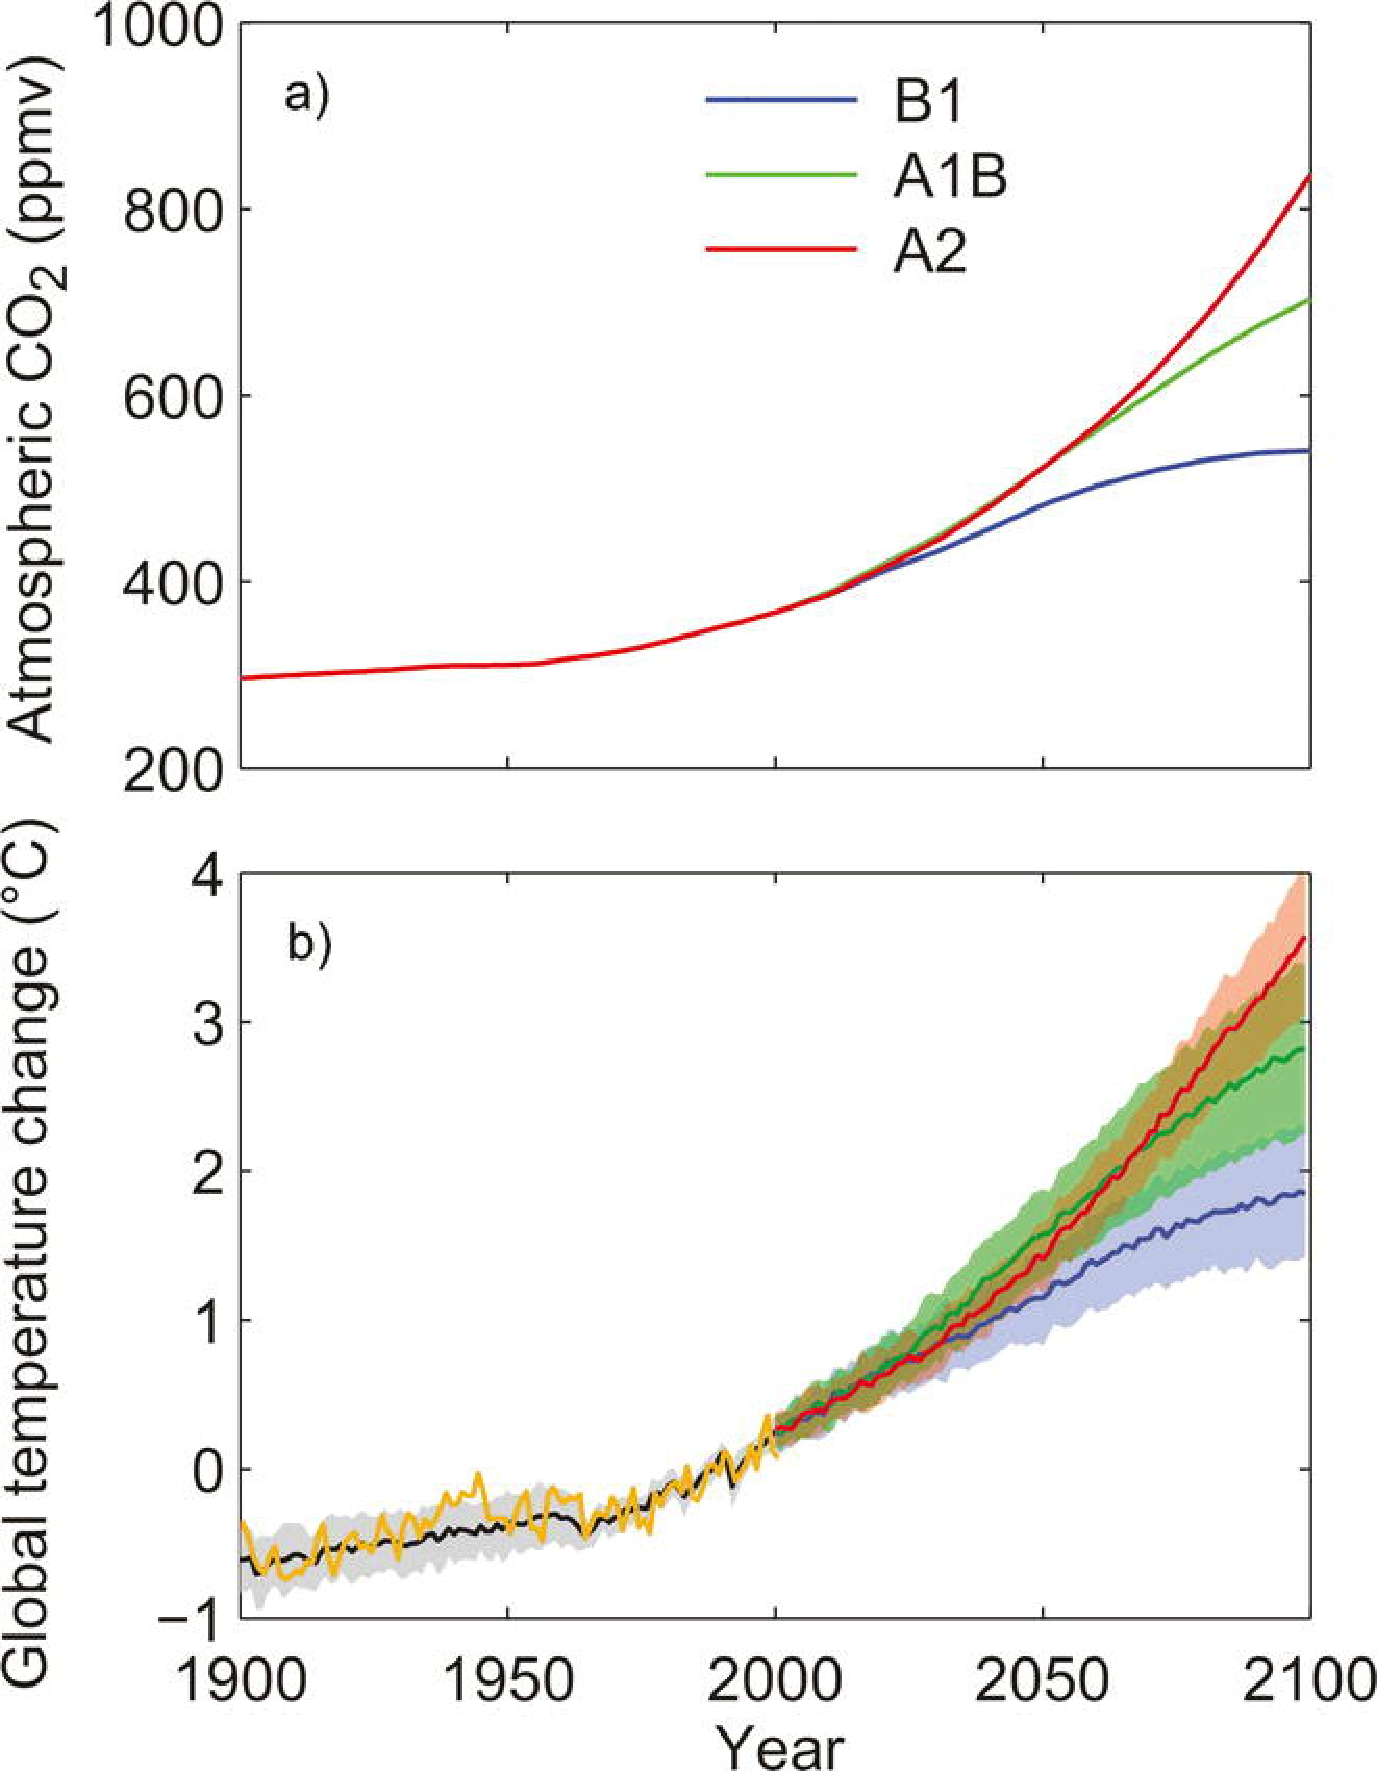
\includegraphics[width=19pc,angle=0]{figure01.pdf}\\
%  \caption{Enter the caption for your figure here.  Repeat as
%  necessary for each of your figures. Figure from \protect\cite{Knutti2008}.}\label{f1}
%\end{figure}
%%%%%%%%%%%%%%%%%%%%%%%%%%%%%%%%%%%%%%%%%%%%%%%%%%%%%%%%%%%%%%%%%%%%%%
%% TABLES
%%%%%%%%%%%%%%%%%%%%%%%%%%%%%%%%%%%%%%%%%%%%%%%%%%%%%%%%%%%%%%%%%%%%%%
%\begin{table}[t]
%\caption{This is a sample table caption and table layout.  Enter as many tables as
%  necessary at the end of your manuscript. Table from Lorenz (1963).}\label{t1}
%\begin{center}
%\begin{tabular}{ccccrrcrc}
%\hline\hline
%$N$ & $X$ & $Y$ & $Z$\\
%\hline
% 0000 & 0000 & 0010 & 0000 \\
% 0005 & 0004 & 0012 & 0000 \\
% 0010 & 0009 & 0020 & 0000 \\
% 0015 & 0016 & 0036 & 0002 \\
% 0020 & 0030 & 0066 & 0007 \\
% 0025 & 0054 & 0115 & 0024 \\
%\hline
%\end{tabular}
%\end{center}
%\end{table}
%
\end{document}